\documentclass{article}

% preambulo:
\usepackage[utf8]{inputenc}
% caracteres utf8 (tildes, enie) sin tener que usar comandos

\usepackage[spanish, es-tabla, es-nodecimaldot]{babel} 
% texto automatico en espaniol
% "tabla" en vez de "cuadro"
% no reemplaza puntos decimales por comas

%% NO AGREGAR PAQUETES ANTES DE ESTO, ES IMPORTANTE QUE BABEL ESTE PRIMERO

%%%%%%%%%%%%%%%%%%%%%%%%%%%%%%%%%
%% PAQUETES EXTRA %%%%%%%%%%%%%%%
%%%%%%%%%%%%%%%%%%%%%%%%%%%%%%%%%

\usepackage{subfiles}

%nuevo
\usepackage[notransparent]{svg}
%

\usepackage{amsmath} % PAQUETES DE MATEMATICA
\usepackage{amsfonts}
\usepackage{amssymb}

%puse esta cosa nueva---
\usepackage{csvsimple}

%-----
\usepackage{steinmetz} % comando \phase{}
\usepackage{units} % permite usar nicefrac
\usepackage{graphicx} % importar imagenes
\usepackage{float} % posicion H para floats
\usepackage[colorinlistoftodos]{todonotes}


\usepackage[a4paper, total={6in, 8in}]{geometry} 
% margenes correctos en subarchivos

\setlength{\parindent}{10pt}			%cuanta sangria al principio de un parrafo
\usepackage{indentfirst}				%pone sangria al primer parrafo de una seccion

\usepackage{listings}

\usepackage{color}

\definecolor{codegreen}{rgb}{0,0.6,0}
\definecolor{codegray}{rgb}{0.5,0.5,0.5}
\definecolor{codepurple}{rgb}{0.58,0,0.82}
\definecolor{backcolour}{rgb}{0.95,0.95,0.92}
 
\lstdefinestyle{mystyle}{
    backgroundcolor=\color{backcolour},   
    commentstyle=\color{codegreen},
    keywordstyle=\color{magenta},
    numberstyle=\tiny\color{codegray},
    stringstyle=\color{codepurple},
    basicstyle=\footnotesize,
    breakatwhitespace=false,         
    breaklines=true,                 
    captionpos=b,                    
    keepspaces=true,                 
    numbers=left,                    
    numbersep=5pt,                  
    showspaces=false,                
    showstringspaces=false,
    showtabs=false,                  
    tabsize=2
}
 
\lstset{style=mystyle}

%%%%%%%%%%%%%%%%%%%%%%%%%%%%%%%%%%%%%%%%%%%%%%%%%%%%%%%%%%%
%% NO AGREGAR PAQUETES DESPUES DE ESTO, ES IMPORTANTE QUE HYPERREF ESTE ULTIMO
\usepackage[colorlinks = true,
            linkcolor = blue,
            urlcolor  = blue,
            citecolor = blue,
            anchorcolor = blue]{hyperref}
%\usepackage[hidelinks]{hyperref} % hipervinculos sin cajitas rojas
\usepackage{bm}


\begin{document}

\newgeometry{} % margenes default para la caratula
% caratula:
\begin{titlepage}
\newcommand{\HRule}{\rule{\linewidth}{0.5mm}}
\center
\mbox{\textsc{\LARGE \bfseries {Instituto Tecnol\'ogico de Buenos Aires}}}\\[1.5cm]
\textsc{\Large 22.85 - Sistemas de Control}\\[0.5cm]


\HRule \\[0.6cm]
{ \Huge \bfseries Trabajo de Laboratorio N$^{\circ}$1: Phase-Locked Loop (PLL) o Lazo de Enganche de Fase}\\[0.4cm] % Title of your document
\HRule \\[1.5cm]


{\large

\emph{Grupo 1}\\
\vspace{3px}

\begin{tabular}{lr} 	
\textsc{M\'aspero}, Martina  & 57120 \\
\textsc{Mestanza}, Joaqu\'in Mat\'ias  & 58288 \\
\textsc{Nowik}, Ariel Santiago  & 58309 \\
\textsc{Panaggio Venerandi}, Guido Martin  & 56214 \\
\textsc{Parra}, Roc\'io  & 57669 \\
\textsc{Regueira}, Marcelo Daniel  & 58300 \\

\end{tabular}

\vspace{20px}

\emph{Profesor}\\
\vspace{3px}
\textsc{Nasini}, V\'ictor Gustavo\\ 	
\vspace{100px}

\begin{tabular}{ll}

Presentado: & xx/09/2019\\

\end{tabular}

}

\vfill

\end{titlepage}

% cambio los margenes para el resto del documento
\newgeometry{left=2.5cm, top=2.5cm, right=2cm, bottom=2cm}

% indice:
\tableofcontents
\newpage



\section{Pasos para la descarga de Lattice Radiant}
Primero entramos al link de descarga de Lattice Radiant


\href{http://www.latticesemi.com/latticeradiant}{http://www.latticesemi.com/latticeradiant}

\subsection{ Elección del sistema operativo}

\begin{figure}[H]
\centering
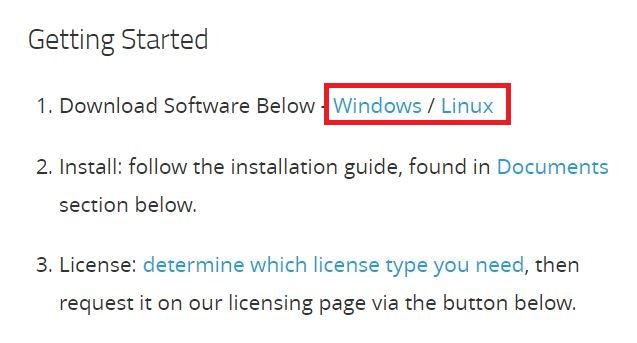
\includegraphics[width=0.4\linewidth]{images/1.JPG}
\caption{Guía de descarga: Paso 1}
\label{fig:step1}
\end{figure}


\subsection{ Ejemplo de selección: caso Windows}

\begin{figure}[H]
\centering
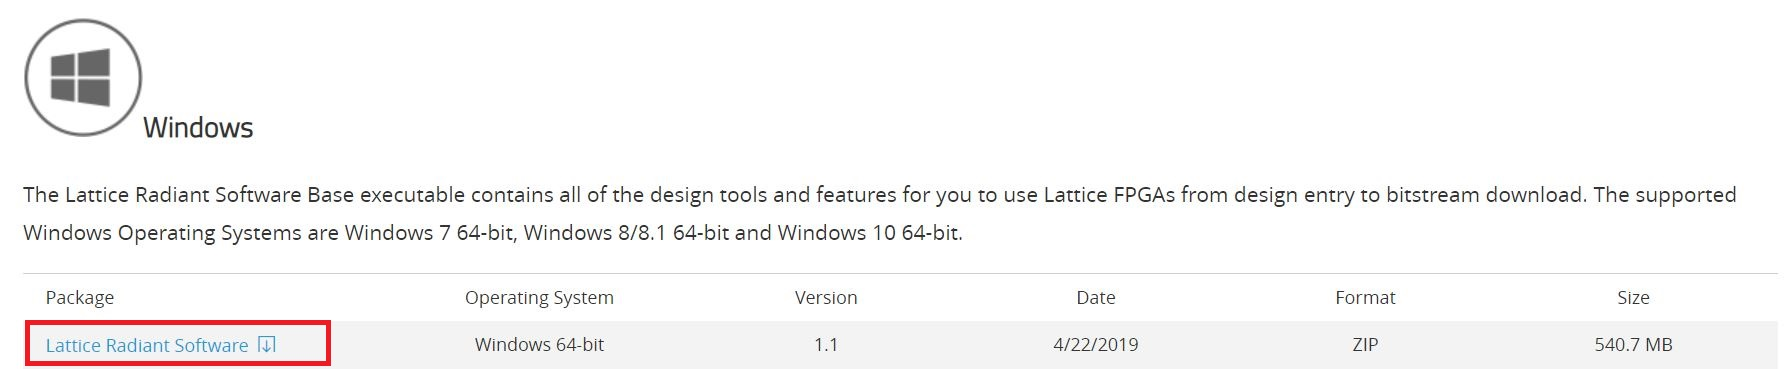
\includegraphics[width=1\linewidth]{images/2.JPG}
\caption{Guía de descarga: Paso 2}
\label{fig:step2}
\end{figure}

\subsection{Sign in request}
Después de haber seleccionado Lattice Radiant Software, nos lleva una página donde para poder entrar tenemos que estar registrados.

\begin{figure}[H]
\centering
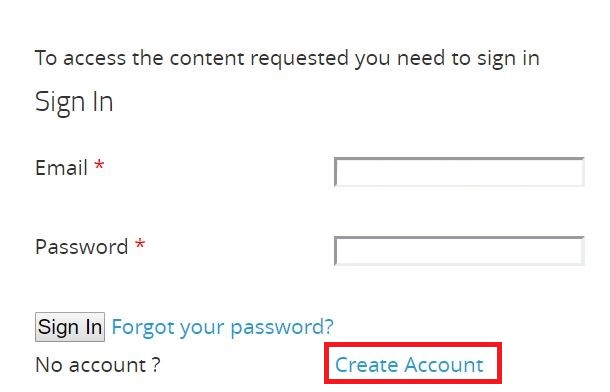
\includegraphics[width=0.4\linewidth]{images/3.JPG}
\caption{Guía de descarga: Paso 3}
\label{fig:step3}
\end{figure}

Para poder seguir, procedemos a registrarnos

\subsection{Registration}
A continuación dejamos una captura de cómo hay que rellenar ciertos campos específicos.

\begin{figure}[H]
\centering
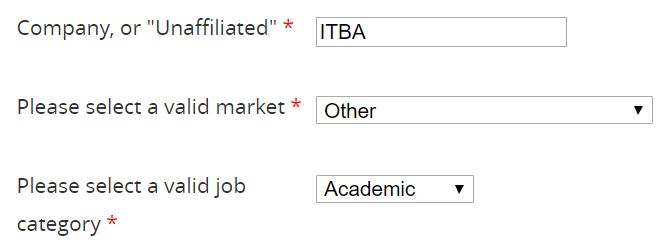
\includegraphics[width=0.4\linewidth]{images/4.JPG}
\caption{Guía de descarga: Paso 4}
\label{fig:step4}
\end{figure}

\subsection{Descarga}
Ahora que tenemos una cuenta, volvemos a la página de lattice para proceder con la descarga. En esa página, aceptamos términos y condiciones, y a continuación clickeamos en Download.

\begin{figure}[H]
\centering
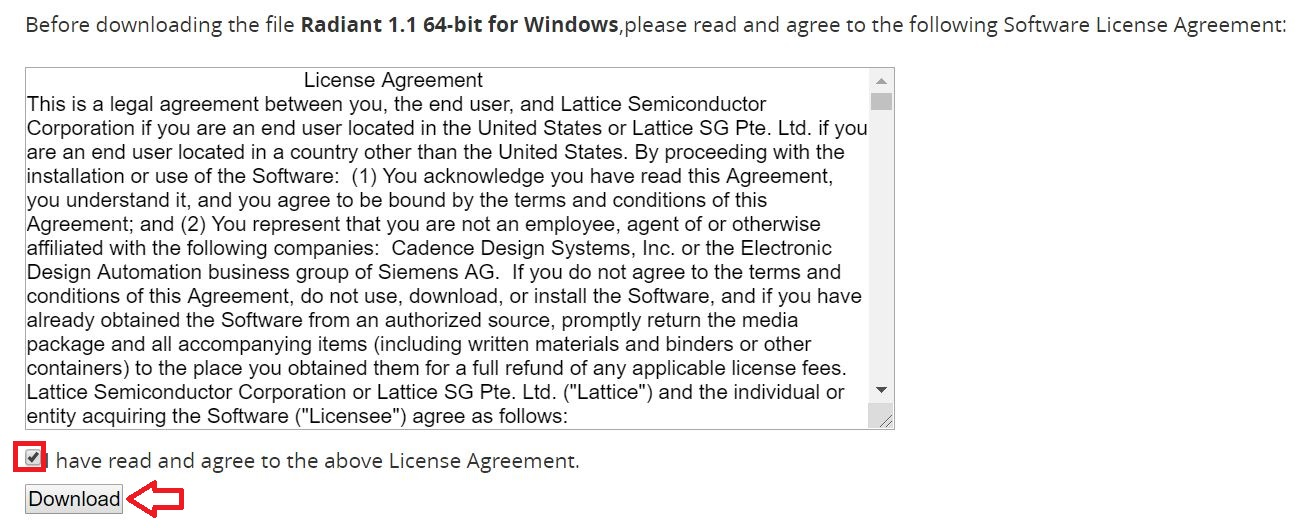
\includegraphics[width=1\linewidth]{images/5.JPG}
\caption{Guía de descarga: Paso 5}
\label{fig:step5}
\end{figure}



\subsection{Licencia}
Para tener una licencia, hay que generar una solicitud en
\href{https://www.latticesemi.com/Support/Licensing}{https://www.latticesemi.com/Support/Licensing}.
En esa página, vamos la parte de Lattice Radiant Software y clickeamos en Request a Free License.

\begin{figure}[H]
\centering
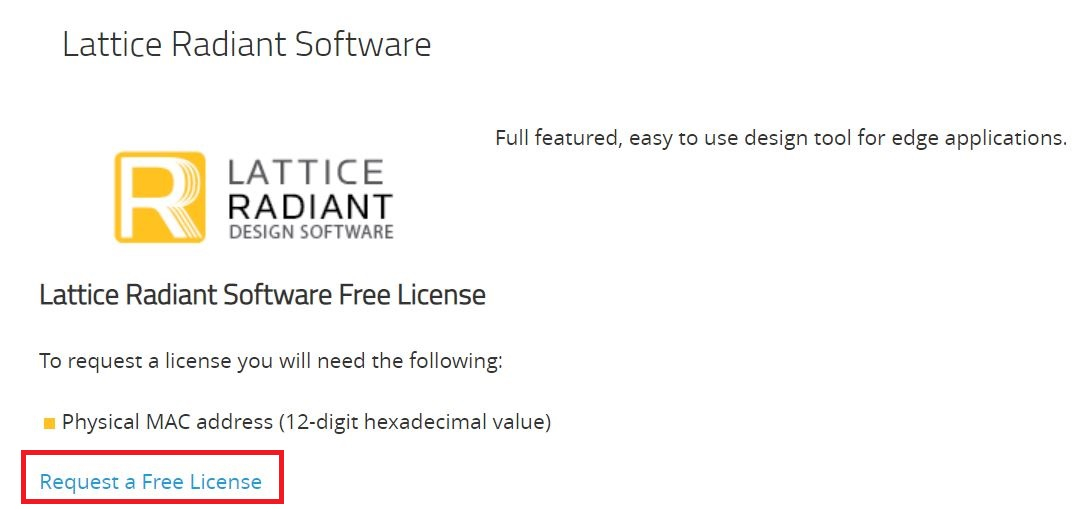
\includegraphics[width=1\linewidth]{images/6.JPG}
\caption{Guía de descarga: Paso 6}
\label{fig:step6}
\end{figure}

El proceso puede demorar 1 día así que hay que procurar no hacerlo a último momento.

\end{document}